\documentclass[a4paper,11pt]{article}

/stock/16_git_repo/library/library.tex

\begin{document}
% Page de garde <<<
../../../../00_resources/page_garde.tex
% >>>
\newpage
\tableofcontents
\newpage

\section{Introduction}

La théorie de l'ordonnancement est une branche non négligeable de l'informatique couvrant un très
grand nombre de problèmes permettant la modélisation d'applications pratiques. Ainsi, des
problématiques aussi diverses que la planification de prises de photographies par satellite,
l'agencement spatial de marchandises dans un entrepôt ou la planification d'une chaîne de production
peuvent être représentées à l'aide de ces problèmes informatiques. Il n'est donc pas étonnant de
de disposer à ce sujet d'une littérature fournie, détaillant nombre de déclinaisons de problèmes
considérés classiques. Cette étude bibliographique, préliminaire au stage, s'inscrit dans cette
démarche et cherche à définir le contexte et les bases nécessaires à l'introduction d'une variante
d'un problème d'ordonnancement très étudié que l'on appelle \isched.

\subsection{Description des problèmes d'ordonnancement}

Nous utiliserons au cours de cette partie les notations communément utilisées pour définir de
manière générale les problèmes d'ordonnancement. Nous serons amenés à définir et utiliser des
notations plus spécifiques au problème considéré.

D'ordinaire, les problèmes d'ordonnancement sont définis par un ensemble de $n$ tâches $\mathcal{T} =
\{T_1, T_2, \dots, T_n\}$ et par un ensemble de $m$ processeurs\footnote{On les appelle aussi des
machines.} $\mathcal{P} = \{\pi_1, \pi_2, \dots, \pi_m\}$. L'ordonnancement consiste à affecter les
tâches $\mathcal{T}$ aux processeurs $\mathcal{P}$ tout en respectant les contraintes définies par
le problème initial. On peut citer deux contraintes largement répendues dans la théorie de
l'ordonnancement :
\begin{enumerate}
    \item chaque processeur peut exécuter au plus une seule tâche à tout instant,
    \item chaque tâche est exécutée par au plus un processeur.
\end{enumerate}

Il paraît important de notifier, qu'il existe des problèmes autorisant l'exécution d'une tâche sur
plusieurs processeurs, la durée d'exécution de la tâche est alors proportionnelle au nombre de
processeurs sur lesquels elle s'exécute. On parle alors de modèles hiérarchiques, mais ces modèles
ne seront pas développés dans le reste de ce manuscrit.

\subsection{Caractérisation des processeurs}

Dans le but de décrire un problème d'ordonnancement, il est important de définir l'environnement des
processeurs, c'est à dire les hypothèses considérées sur les machines. Au cours de ce rapport, seul
le modèle des processeurs parallèles, exécutant tous les mêmes fonctions, sera considéré. Pour la
découverte du modèle des processeurs dédiés, spécialisés dans l'exécution de certaines fonctions,
nous invitons les intéressés à la lecture du livre~\cite{blazewicz_handbook_2007}.

Les processeurs parallèles se décomposent en trois catégories :
\begin{enumerate}
    \item identiques : tous les processeurs de $\mathcal{P}$ admettent la même vitesse de traitement
    \item uniformes : les vitesses de traitement diffèrent mais la vitesse de traitement est
        proportionnelle à un coefficient propre à chaque machine appelé facteur d'accélaration
    \item généraux : les vitesses de traitement dépendent des tâches à effectuer
\end{enumerate}

À nouveau nous ne considérerons qu'une seule catégorie, les problèmes nous intéressant ne portent
que sur des processeurs identiques.

\subsection{Caractérisation des tâches}

Généralement, en ordonnancement, une tâche est définie par cinq paramètres :
\begin{enumerate}
    \item un vecteur de temps d'exécution $p_j = ^t(p_{j1}, p_{j2}, \dots, p_{jm})$ où $p_{ji}$
        représente le temps nécessaire à l'exécution de la tâche $j$ sur la machine $i$. Dans le cas
        de machines identiques et uniformes, ce vecteur ne présente qu'une seule composante,
    \item une date de disponibilité $r_j$, désignant la date à partir de laquelle la tâche est prête
        à être exécutée,
    \item une date d'échéance $d_j$, désignant la date souhaitée à laquelle la tâche $j$ devrait
        être exécutée,
    \item une date de fin impérative$\widetilde{d_j}$, date à laquelle la tâche doit obligatoirement être exécutée,
    \item un poids $w_j$, représentant l'urgence relative de la tâche.
\end{enumerate}

Les tâches ainsi définies peuvent être soumises à certaines contraintes, telles que des contraintes
de précédences, imposant que la date d'exécution d'une exécution soit ultérieure à la complétion
d'un ensemble de tâches tierces.

Si l'on considère le graphe, que nous appellerons le graphe d'exclusion, qui à chaque tâche associe
un sommet, et tel qu'il existe une arête entre deux sommets si deux taches ne peuvent être affectée
à la même machine, il est alors possible d'imposer des contraintes structurelles à ce graphe. 

\subsection{Notation à trois champs}

La multitude de problèmes d'ordonnancement énoncée précédemment a conduit à la mise en place d'une
notation synthétique permettant la description de ces schémas. Nous nous proposons de reprendre la
notation introduite par Graham~\cite{graham} et B\l a\.zewicz~\cite{blazewicz}. 

Pour cette notation, il nous faut introduire trois paramètres $\alpha, \beta, \gamma$. Détaillons
ces paramètres :
\begin{enumerate}
    \item le paramètre $\alpha$ permet de caractériser l'environnement des processeurs. $\alpha \in
        \left\{ P, \bar{P}, P_m, Q, R \right\}$, avec :
        \begin{itemize}
            \item $P$ : les processeurs sont identiques et leur nombre est une entrée du problème,
            \item $\bar{P}$ : les processeurs sont identiques, mais leur nombre est dit suffisant ou
                non borné,
            \item $P_m$ : les processeurs sont identiques et leur nombre est fixé,
            \item $Q$ : les processeurs sont uniformes
            \item $R$ : les processeurs dont généraux
        \end{itemize}
    \item le paramètre $\beta$ permet de définir le type d'application et ses caractéristiques
        telles que les contraintes de précédence ou les durées d'exécution des tâches. Nous écrirons
        ce paramètre sous la forme $\beta = \beta_1\beta_2\beta_3$ avec :
        \begin{itemize}[label=$\bullet$]
            \item $\beta_1$ représentant les contraintes de précédence :
                \begin{itemize}
                    \item $\beta_1 = prec$ : le graphe de précédence est un graphe quelconque
                    \item $\beta_1 = arbre$ : le graphe de précédence est un arbre
                    \item[$\vdots$]
                    \item $\beta_1 = .$ : les tâches sont indépendantes
                \end{itemize}
            \item $\beta_2$ représentant les temps d'exécution des tâches :
                \begin{itemize}
                    \item $\beta_2 = p_j = 1$ : les tâches sont unitaires, leur durée est égale à
                        $1$
                    \item $\beta_2 = .$ : les durées des tâches sont données par le graphe
                \end{itemize}
            \item $\beta_3$ représentant les propriétés structurelles du graphe d'exclusion :
                \begin{itemize}
                    \item $\beta_3 = inter$ : le graphe d'exclusion est un graphe d'intervalles
                    \item $\beta_3 = .$ : le graphe d'exclusion est un graphe vide (sans arêtes)
                \end{itemize}<++>
        \end{itemize}
    \item le paramètre $\gamma$ représente quant à lui définit la fonction objectif que l'on
        cherchera à optimiser.
\end{enumerate}

\subsection{Motivations}

Les problèmes considérés tout au long de ce rapport s'inscrivent dans la branche de l'ordonnancement
appelée \isched, dans cette branche le début et la fin de chaque tâche $j$ sont
fixés, la tâche est donc représentable par un intervalle $\left[ \st{j}, \ct{j} \right]$ et un poids
$w_j$. 

Il est usuel, pour cette catégorie de problème,  de considérer un ensemble de tâches tel qu'il est
impossible de pouvoir assigner à chaque tâche une machine, l'optimisation se fait alors en
maximisant le poids de l'ensemble des tâches affectées à une machine.

Le but de ce stage est d'étudier une nouvelle fonction objectif pour ces problèmes cherchant à
optimiser la flexibilité de l'ordonnancement produit en minimisant la fragmentation de
l'ordonnancement produit.

\section{État de l'art}

Au cours de cette section nous présenterons, dans un premier temps, le problème \bisched ainsi qu'un
certain nombre de résultats sur ce dernier. Puis nous introduirons quelques unes des nombreuses
variantes de ce problème et là aussi nous décrirons quelques résultats que l'on peut trouver dans la
littérature. Ces problèmes ont été choisis pour les similitudes qu'ils présentent avec le problème
étudié.

\subsection{Le problème \bisched}

Étant donnés un ensemble de $n$ tâches $\mathcal{T} = \left\{
j_1, j_2, \dots, j_n \right\}$ représentés par un ensemble de $n$ intervalles $\mathcal{I} = \{
[ \st{j_1}, \ct{j_1} ], [ \st{j_2}, \ct{j_2} ], \dots, [ \st{j_n},
\ct{j_n} ] \}$ avec $\ct{j_i} > \st{j_i}$ pour $i = 1, \dots, n$, et un ensemble de
machines $\mathcal{M} = \left\{ m_1, m_2, \dots, m_k \right\}$, le but est alors de trouver un
ordonnancement minimisant le nombre de machines utilisées par ce dernier.

On peut définir la notation à trois champs de ce problème :
\begin{center}
    $\bar{P} \Big| . . inter \Big| \min \#(\mathcal{M})$
\end{center}

Ce problème, comme tous les autres problèmes d'\isched, est fortement lié à la notion de graphe
d'intervalles. Un graphe d'intervalles est un graphe tel que ses sommets sont représentables par
des intervalles et il existe une arête entre deux sommets si et seulement si les intervalles
associés à ces sommets s'intersectent lorsqu'ils sont représenté sur la ligne des réels. Un exemple
de graphe d'intervalles est donné à la
figure~\ref{fig:ex_gint}. Il est facile de voir que si l'on considère le graphe représentant les
tâches qui ne peuvent s'exécuter sur la même machine, on obtient alors un graphe d'intervalle.

\begin{figure}
    \centering
    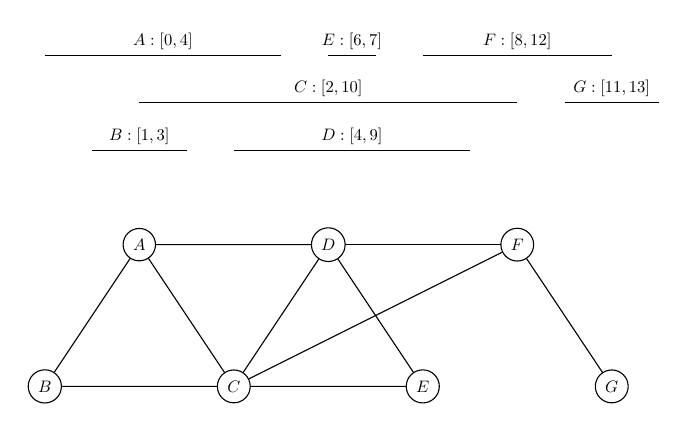
\begin{tikzpicture}[noeud/.style={draw=black, circle}, scale=0.6, every node/.style={transform shape}]
        \draw[-] (0,  0) to node[above] {$A : [0,4]$} (5,0);
        \draw[-] (1, -2) to node[above] {$B : [1,3]$} (3,-2);
        \draw[-] (2, -1) to node[above] {$C : [2, 10]$} (10, -1);
        \draw[-] (4, -2) to node[above] {$D : [4, 9]$} (9, -2);
        \draw[-] (6,  0) to node[above] {$E : [6,7]$} (7,0);
        \draw[-] (8,  0) to node[above] {$F : [8,12]$} (12,0);
        \draw[-] (11, -1) to node[above] {$G : [11, 13]$} (13, -1);

        \node[noeud] (A) at (2, -4) {$A$};
        \node[noeud] (B) at (0, -7) {$B$};
        \node[noeud] (C) at (4, -7) {$C$};
        \node[noeud] (D) at (6, -4) {$D$};
        \node[noeud] (E) at (8, -7) {$E$};
        \node[noeud] (F) at (10, -4) {$F$};
        \node[noeud] (G) at (12, -7) {$G$};

        \draw[-] (A) to (B);
        \draw[-] (A) to (C);
        \draw[-] (A) to (D);

        \draw[-] (B) to (C);
        
        \draw[-] (C) to (D);
        \draw[-] (C) to (E);
        \draw[-] (C) to (F);

        \draw[-] (D) to (E);
        \draw[-] (D) to (F);

        \draw[-] (F) to (G);
    \end{tikzpicture}
    \caption{Un exemple de graphe d'intervalles}
    \label{fig:ex_gint}
\end{figure}

Pour le problème \bisched, le rapport avec les graphe d'intervalles ne s'arrête pas là, en effet, le
problème a été démontré équivalent à la recherche du nombre chromatique du graphe d'intervalle
associé au problème~\cite{golumbicalgorithmic}. Le nombre chromatique d'un graphe étant le plus
petit nombre de couleurs nécessaires à la coloration d'un graphe. Dans la mesure où le problème de
coloration de graphes d'intervalles est polynomiale, le problème \bisched l'est aussi, ainsi Ford et
Fulkerson ont proposé en 1962, un algorithme s'exécutant en $O(n^2)$
opérations~\cite{ford1962network}. Depuis d'autres méthodes ont été proposées notamment par Gupta et
al. ayant une complexité en $O(n\log n)$ opérations et qu'ils ont démontrée comme atteignant la
meilleur complexité possible~\cite{gupta_optimal_1978}.

L'algorithme repose sur une observation simple : le nombre minimal de couleur nécessaire à la
coloration du graphe d'intervalle est égal à la taille de la plus grande clique de ce graphe, or une
clique de taille $k$ dans le graphe associé à l'ensemble des tâches correspond à une durée pendant
laquelle $k$ intervalles s'intersectent deux à deux. Ainsi, en parcourant les dates de début des tâches par
ordre de dates de début, et en assignant cette tâche à une machine, ayant déjà été utilisée
précédemment, l'algorithme s'assure qu'une nouvelle machine est utilisée lorsque le nombre de
tâches s'intersectant deux à deux est supérieur aux nombres de machines déjà utilisées. Dans ce cas
le nombre de couleur déjà utilisé pour colorer le graphe est inférieur à la taille de la clique
courante (et donc nécessairement de la plus grande clique).

Un algorithme distribué a été mis au point par Dekel et Sani~\cite{dekel1983parallel}, permettant la
résolution de ce problème en $O(\log n)$ moyennant $O(n^2 / \log n)$ machines.

\subsection{Quelques variantes de ce problème}

Il existe beaucoup de déclinaisons du problème \bisched considérant une autre fonction objectif,
modifiant l'environnement des processeurs, ou encore introduisant de nouvelles notions permettant
d'augmenter l'expressivité du modèle. Parmis ces variantes, nous en avons choisi deux permettant de
définir le contexte de notre modèle.

\subsubsection{Nombre de machines fixé}

Cette variante, contrairement au problème originel, fixe le nombre de machines pouvant exécuter les
tâches et cherche un ordonnancement permettant de maximiser la somme du poids des tâches affectées à
une machine. Le poids $w_j$ d'une tâche $j$ peut être vu comme le profit généré par l'exécution de
la tâche $j$, le problème cherche alors à maximiser les gains.

Nous noterons ce problème :
\begin{center}
    $P \Big| . . inter \Big| \max \sum w_j : j$ est affectée à une machine de $\mathcal{M}$
\end{center}

Sans contraintes supplémentaires, le problème est polynomial, Arkin et Silverberg ayant proposé en
1986 un algorithme s'exécutant en $O(n^2 \log n)$ opérations~\cite{arkin_scheduling_1987}. Cet
algorithme repose sur la même observation que celui de Gupta et al. précédemment présenté : il faut
exactement $p$ couleurs pour colorer une clique de taille $p$. Donc étant donné $\mathcal{M}=\left\{
m_1, m_2, \dots, m_k \right\}$ un ensemble de $k$ machines, pour toutes les cliques de taille
$p$ supérieure à $k$, l'algorithme cherche à supprimer les $p -k$ sommets de la clique présentant
le plus petit profit. Ces sommets sont identifiés à l'aide d'un algorithme de flot de coût minimum
dans un graphe construit à partir des cliques du graphes d'intervalles de départ.

Cet algorithme a donc la particularité de trouver un ordonnancement de profit maximal, non pas en
trouvant les tâches à affecter, mais en trouvant celle à ne pas affecter.

À présent, considérons ce même problème, à ceci prêt : chaque tâche $j$ de $\mathcal{T}$ va se voir
attribuer un ensemble de machines $\mathcal{M}_j \subseteq \mathcal{M}$ représentant l'ensemble des
machines sur lesquelles la tâche $j$ peut être exécutée.

Ce problème devient alors \npc si le nombre de machine dans chaque sous-ensemble $\mathcal{M_j}$ est
supérieur ou égal à $3$~\cite{arkin_scheduling_1987}, la preuve se faisant par une réduction depuis
le problème \textsc{$3-$SAT}. Un algorithme exprimé sous forme de programmation dynamique a été
décrit dans ce même article, il s'exécute en $O(n^{k+1})$.

Bhatia et al. ont proposé une $(1 - 1/\varepsilon)-$approximation
randomisée~\cite{bhatia2003algorithmic} basée sur de la programmation linéaire permettant la
résolution de ce problème. De plus de nombreuses heuristiques ont été introduite pour répondre à ce
problème, nous renvoyons les intéressés à la lectures des articles~\cite{kroon1995exact}
et~\cite{gabrel1995scheduling}.

\subsubsection{Indisponnibilité de machines}

Une seconde extension au problème \bisched est une variante introduisant des périodes au cours
desquelles certaines machines seront dites indisponibles et donc pendant lesquelles elles ne
pourront effectuer aucun calcul. La machine entrant en indisponibilité ne doit avoir aucune tâche en
curt d'exécution, un ordonnancement présentant une intersection entre une tâche et une
indisponibilité n'est donc pas un ordonnancement valide.

Comme vu précédemment, les problèmes d'ordonnancement d'intervalles ont un lien fort avec les
graphes d'intervalles, \bisched étant équivalent au problème de coloration sur ces derniers. Il
existe une catégorie de graphe, à savoir les graphes à arcs circulaires qui est le
graphe d'intersection d'un ensemble d'arcs de cercle, dont le problème de coloration est équivalent
au problème avec machines indiponibles.

\begin{figure}
    \centering
    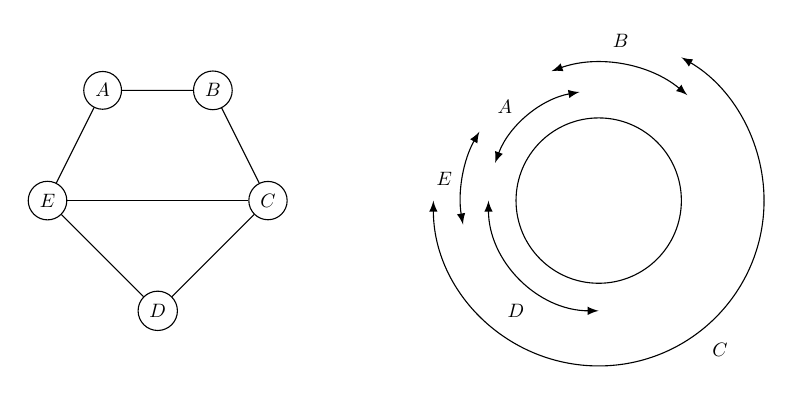
\begin{tikzpicture}[n/.style={draw=black, circle}, scale=0.7, every node/.style={transform shape}, >=latex]
        \node[n] (A) at (1, 4) {$A$};
        \node[n] (B) at (3, 4) {$B$};
        \node[n] (C) at (4, 2) {$C$};
        \node[n] (D) at (2, 0) {$D$};
        \node[n] (E) at (0, 2) {$E$};

        \draw[-] (A) to (B);
        \draw[-] (A) to (E);

        \draw[-] (B) to (C);

        \draw[-] (C) to (D);
        \draw[-] (C) to (E);

        \draw[-] (D) to (E);

        \draw (10,2) circle (1.5cm);
        \draw[rotate around={100:(10,2)}, <->] (12, 2) arc (0:60:2cm);
        \draw[rotate around={150:(10,2)}, <->] (12.5, 2) arc (0:40:2.5cm);
        \draw[rotate around={180:(10,2)}, <->] (12, 2) arc (0:90:2cm);
        \draw[rotate around={180:(10,2)}, <->] (13, 2) arc (0:240:3cm);
        \draw[rotate around={ 50:(10,2)}, <->] (12.5, 2) arc (0:60:2.5cm);

        \node (a) at (8.3, 3.7) {$A$}; 
        \node (b) at (10.4, 4.9) {$B$}; 
        \node (c) at (12.2, -0.7) {$C$}; 
        \node (d) at (8.5, 0) {$D$}; 
        \node (e) at (7.2, 2.4) {$E$}; 
        
    \end{tikzpicture}
    \caption{Exemple de graphe à arcs circulaires}
    \label{fig:fig_ex_ac}
\end{figure}


\newpage
\appendix
\bibliographystyle{plain}
\bibliography{biblio}


\end{document}
